\section{Punto de Vista de Estrategia}

El punto de vista de estrategia de la parte ArchiMate de cualquier proyecto que se esté realizando es crucial y fundamental, no solo por el hecho como su nombre lo indica, de trazar una estrategia a seguir en el transcurso y desarrollo del proyecto, sino que brinda una visión mucho más amplia que esto, este punto de vista como continuación al punto de vista de motivación, recoge los resultados de este punto de vista, los cuales se transforman en los outputs o resultados que se quieren con el proyecto y a partir de los mismos se desglosa todo lo que tiene que ver con la estrategia, es decir, que se va a realizar, como lo va a hacer y con ayuda de quien o de que además, de mencionar que recursos se requieren para poder tener el resultado mencionado.

\subsection{Modelo de Estrategia}
\begin{figure}[h!]
	\centering
	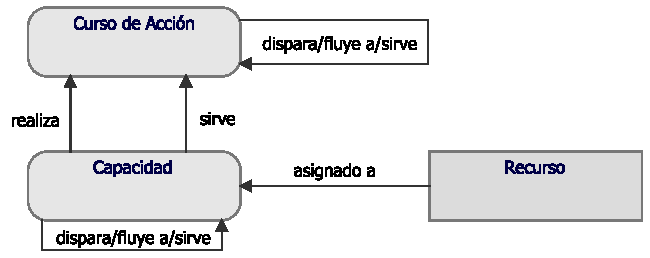
\includegraphics[width=.8\linewidth]{imgs/caso/Estrategia}
	\caption{Modelo Mapa de Capacidad}
\end{figure}

El modelo de estrategia del punto de vista de estrategia, se compone de cuatro elementos principales, los cuales son: el primer elemento y como principal, es el resultado, el cual proviene de la capa de motivación y se convierte en el mismo output, el segundo componente es el centro del punto de vista, ya que es el curso de acción o estrategia a tomar para llegar al resultado deseado, de ahí se derivan que capacidades se necesitan para desarrollar esa estrategia o ese curso de acción y finalmente se especifican los recursos necesarios para lograr el objetivo deseado.

\newpage

\subsection{Caso de Estrategia}

\subsubsection{Resultado 1: Mejores Investigadores e Investigaciones}

\begin{figure}[h!]
	\centering
	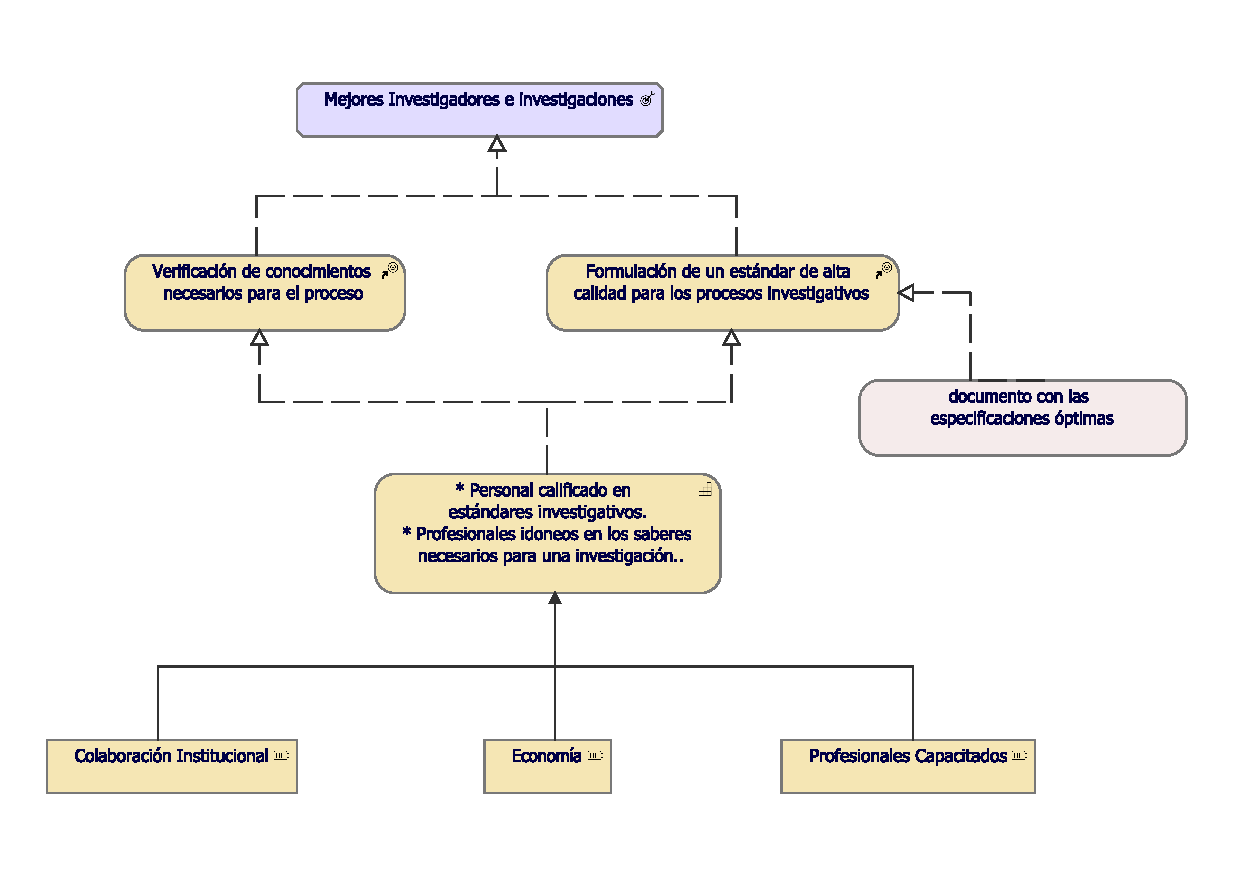
\includegraphics[width=1\linewidth]{imgs/modelo/estrategia/Estrate/EstrategiaResult1.pdf}
	\caption{Caso Estrategia (Resultado 1)}
\end{figure}

El resultado 1 se refiere a Mejores Investigadores e investigaciones, este es un output o salida fundamental esperada en el proyecto planteado, para el cual se realizan dos cursos de acción con el fin de cumplir el objetivo de llevar a buen término este resultado, el primer curso de acción es la Verificación de conocimientos necesarios para el proceso investigativo y el segundo es la formulación de un estándar de alta calidad para los procesos investigativos,  para este ultimo curso de acción se requiere un documento con las especificaciones óptimas para ese estándar que se necesita. Para cumplir con estas estrategias, se requiere unas capacidades fundamentales que se pueden resumir en: personal calificado en estándares investigativos y profesionales idóneos en los saberes necesarios para una investigación y, finalmente se mencionan los recursos que se necesitan para llevar a cabo el desarrollo de las estrategias que den como resultado el output esperado, estos son: colaboración institucional, economía y profesionales capacitados.


\clearpage
\subsubsection{Resultado 2: Generación de Estudiantes de Alta Calidad}

\begin{figure}[h!]
	\centering
	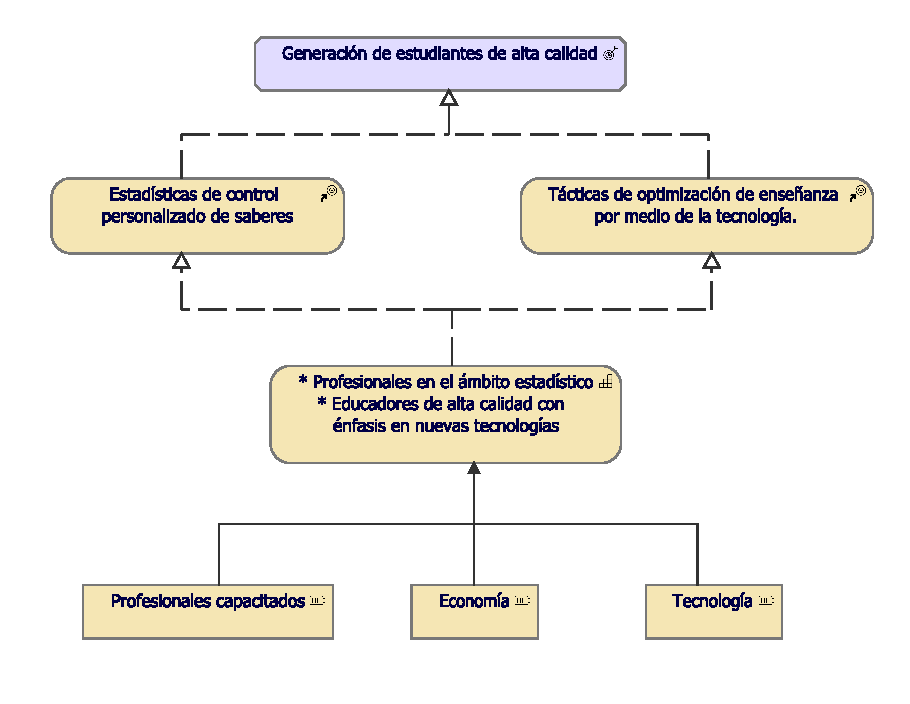
\includegraphics[width=.8\linewidth]{imgs/modelo/estrategia/Estrate/EstrategiaResult2.pdf}
	\caption{Caso Estrategia (Resultado 2)}
\end{figure}

El segundo resultado derivado de la capa motivacional es la generación de estudiantes de alta calidad, el cual es el objetivo principal y fundamental del proyecto en desarrollo, para esto se requieren una serie de estrategias adecuadas que posibiliten la obtención de dicho resultado, estas estrategias son: en primer lugar la creación de estadísticas de control personalizado de saberes y en segundo lugar la tácticas de optimización de enseñanza por medio de la tecnología. Ya teniendo las estrategias a tomar, se debe definir que capacidades se requieren para cumplir con el objetivo, estas capacidades son: profesionales en el ámbito estadístico y educadores de alta calidad con énfasis en nuevas tecnologías. y finalmente, se requiere saber cuales son los recursos necesarios para realizar la estrategia o estrategias planteadas, en este caso son dos estrategias, estos recursos son: profesionales capacitados, economía y tecnología.

\clearpage